\documentclass{article}
\usepackage{graphicx}
\usepackage{listings}
\usepackage{amsmath}
\usepackage[left=2cm, right=2cm]{geometry}
\title{Hand-in 2}
\author{Michael Iversen\\
Student ID: 201505099}

% Default fixed font does not support bold face
\DeclareFixedFont{\ttb}{T1}{txtt}{bx}{n}{10} % for bold
\DeclareFixedFont{\ttm}{T1}{txtt}{m}{n}{10}  % for normal

% Custom colors
\usepackage{color}
\definecolor{deepblue}{rgb}{0,0,0.5}
\definecolor{deepred}{rgb}{0.6,0,0}
\definecolor{deepgreen}{rgb}{0,0.5,0}

\usepackage{listings}
\usepackage{lipsum}
% Python style for highlighting
\newcommand\pythonstyle{\lstset{
		language=Python,
		basicstyle=\ttm,
		morekeywords={self},              % Add keywords here
		keywordstyle=\ttb\color{deepblue},
		emph={MyClass,__init__},          % Custom highlighting
		emphstyle=\ttb\color{deepred},    % Custom highlighting style
		stringstyle=\color{deepgreen},
		showstringspaces=false
}}

% Python environment
\lstnewenvironment{python}[1][]
{
	\pythonstyle
	\lstset{#1}
}
{}


\begin{document}
\maketitle
\section*{PART I: Derivative}
When implementing the neural network, we apply the following loss function for a single data point,
\begin{align*}
	L(z) = - \sum_{i=1}^k y_i \ln(\mathrm{softmax}(z)_i).
\end{align*}
Let $y_j = 1$ be the correct label and $y_i = 0$ for $i \neq j$. The loss function can be rewritten as,
\begin{align*}
	L(z) = - \ln(\mathrm{softmax}(z)_j).
\end{align*}
In this section, we determine the derivative of the loss function with respect to all entries of $z$: $\frac{\partial L}{\partial z_i}$.
We determine the derivative by direct calculation.
\begin{align*}
	\frac{\partial L}{\partial z_i} &= \frac{\partial }{\partial z_i} \left[ - \ln \left( \frac{e^{z_j}}{\sum_{a=1}^k e^{z_a}} \right) \right] \\
	\intertext{Applying the chain rule and quotient rule, we find,}
	&= - \frac{\sum_{a=1}^k e^{z_a}}{e^{z_j}} \cdot \frac{\delta_{ij} e^{z_j} \big(\sum_{a=1}^k e^{z_a}\big) - e^{z_j} \big(\sum_{a=1}^k \delta_{ia}e^{z_a}\big)}{\big(\sum_{a=1}^k e^{z_a}\big)^2} \\
	&= - \frac{\sum_{a=1}^k e^{z_a}}{e^{z_j}} \cdot \frac{\delta_{ij} e^{z_j} \big(\sum_{a=1}^k e^{z_a}\big) - e^{z_j} e^{z_i}}{\big(\sum_{a=1}^k e^{z_a}\big)^2} \\
	&= - \delta_{ij} + \frac{e^{z_i}}{\sum_{a=1}^k e^{z_a}} \\
	&= - \delta_{ij} + \mathrm{softmax}(z_i).
\end{align*}
In total, the derivative is given by the simple expression, $\frac{\partial L}{\partial z_i}  = - \delta_{ij} + \mathrm{softmax}(z_i)$.

\section*{PART II: Implementation and test}
\subsection*{Implementation}
The implementation of the forward pass and backward pass are shown in the code snippet at the end of this section. 

In the forward pass, the mean negative log likelihood is computed and saved as the variable ``cost''. 
Next, the weight decay is computed and saved as the variable ``weight\_decay''. 
Finally, the total loss is computed as the sum of the mean negative log likelihood and the weight decay: ``L = cost + weight\_decay''.
The intermediate results are stored since these will be reused in the backward pass.
I use the notation that ``X1\_W1'' corresponds to $X_1 \cdot W_2$ and ``X1\_W1\_b1'' corresponds to $X_1 \cdot W_1 + b_1$.
To simplify notation, I denote $\mathrm{relu}(X_1 \cdot W_1 + b_1)$ by ``X2''.
Using this notation, the quantity $\mathrm{relu}(X_1 \cdot W_1 + b_1) \cdot W_2$ is identified with ``X2\_W2''.
I also use the notation ``z'' for $\mathrm{relu}(X_1 \cdot W_1 + b_1) \cdot W_2 + b_2$.
I use the variables ``W1\_squared'', ``W2\_squared'' and ``W1\_W2\_sum'' to store intermediate values when computing the weight decay.

In the backward pass, I use the notation ``d\_x'' to signify the Jacobian matrix of the cost function with respect to the variable ``x''.
For instance, the variable ``d\_z'' corresponds to $\frac{\partial L}{\partial \vec z}$, ``d\_b2'' corresponds to $\frac{\partial L}{\partial \vec b_2}$, etc. 
The backpropagation begins by using the expression from PART I to compute ``d\_z''. Next, the Jacobian of the loss function with respect to $W_1$, $b_1$, $W_2$ and $b_2$ may be computed by iteratively performing backpropgation. I illustrate this procedure by going through a few steps.
First, the Jacobian matrix with respect to ``X2\_W2'' is identical to the Jacobian matrix with respect to ``z'' because ``z'' is simply the sum of ``X2\_W2'' and ``b2''.
Similarly, ``d\_b2'' is determined by summing ``d\_z'' over the rows because ``b2'' is added to each data point in the computational graph.
Next, ``d\_X2'' are computed using the following formula ``d\_X2 = d\_X2\_W2 @ W2.transpose()'' (taken from https://cs231n.github.io/optimization-2/).
The remaining quantities are calculated using similar methods.
\begin{python}
@staticmethod
def cost_grad(X, y, params, c=0.0):
	W1 = params['W1']
	b1 = params['b1']
	W2 = params['W2']
	b2 = params['b2']
	labels = one_in_k_encoding(y, W2.shape[1])
	
	# ----------- FORWARD PASS ----------- #
	# Cost
	X1_W1 = X @ W1
	X1_W1_b1 = X1_W1 + b1
	X2 = relu(X1_W1_b1)
	X2_W2 = X2 @ W2
	z = X2_W2 + b2
	cost = - np.sum(labels * np.log(softmax(z)))
	
	# Weight decay
	W1_squared = W1 ** 2
	W2_squared = W2 ** 2
	W1_W2_sum = np.sum(W1_squared) + np.sum(W2_squared)
	weight_decay = c * W1_W2_sum
	
	# Total loss
	L = cost + weight_decay
	
	#  ----------- BACKWARD PASS ----------- #
	# Cost
	d_z = - labels + softmax(z)
	d_X2_W2 = d_z
	d_b2 = np.sum(d_z, axis=0, keepdims=True)
	d_X2 = d_X2_W2 @ W2.transpose()
	d_W2 = X2.transpose() @ d_X2_W2
	d_X1_W1_b1 = d_X2 * np.heaviside(X1_W1_b1, 0)
	d_X1_W1 = d_X1_W1_b1
	d_b1 = np.sum(d_X1_W1_b1, axis=0, keepdims=True)
	d_W1 = X.transpose() @ d_X1_W1
	
	# Weight decay
	d_W1_weight = c * 2 * W1
	d_W2_weight = c * 2 * W2
	
	d_w1 = d_W1 + d_W1_weight
	d_w2 = d_W2 + d_W2_weight
	return L, {'d_w1': d_w1, 'd_b1': d_b1, 'd_w2': d_w2, 'd_b2': d_b2}
\end{python}

\subsection*{Tests}
The model is trained on the MNIST data set using mini batch stochastic gradient descent. The insample accuracy is $\mathrm{Acc}_\mathrm{in} = 0.998$ and the validation accuracy is $\mathrm{Acc}_\mathrm{val} = 0.983$. 
Figure \ref{fig:error} illustrates the insample and validation error as a function of epochs in the left plot and insample and validation accuracy as a function of epochs in the right plot.
We see that the neural network achieves very high accuracy after just a few epochs.
\begin{figure}
	\centering
	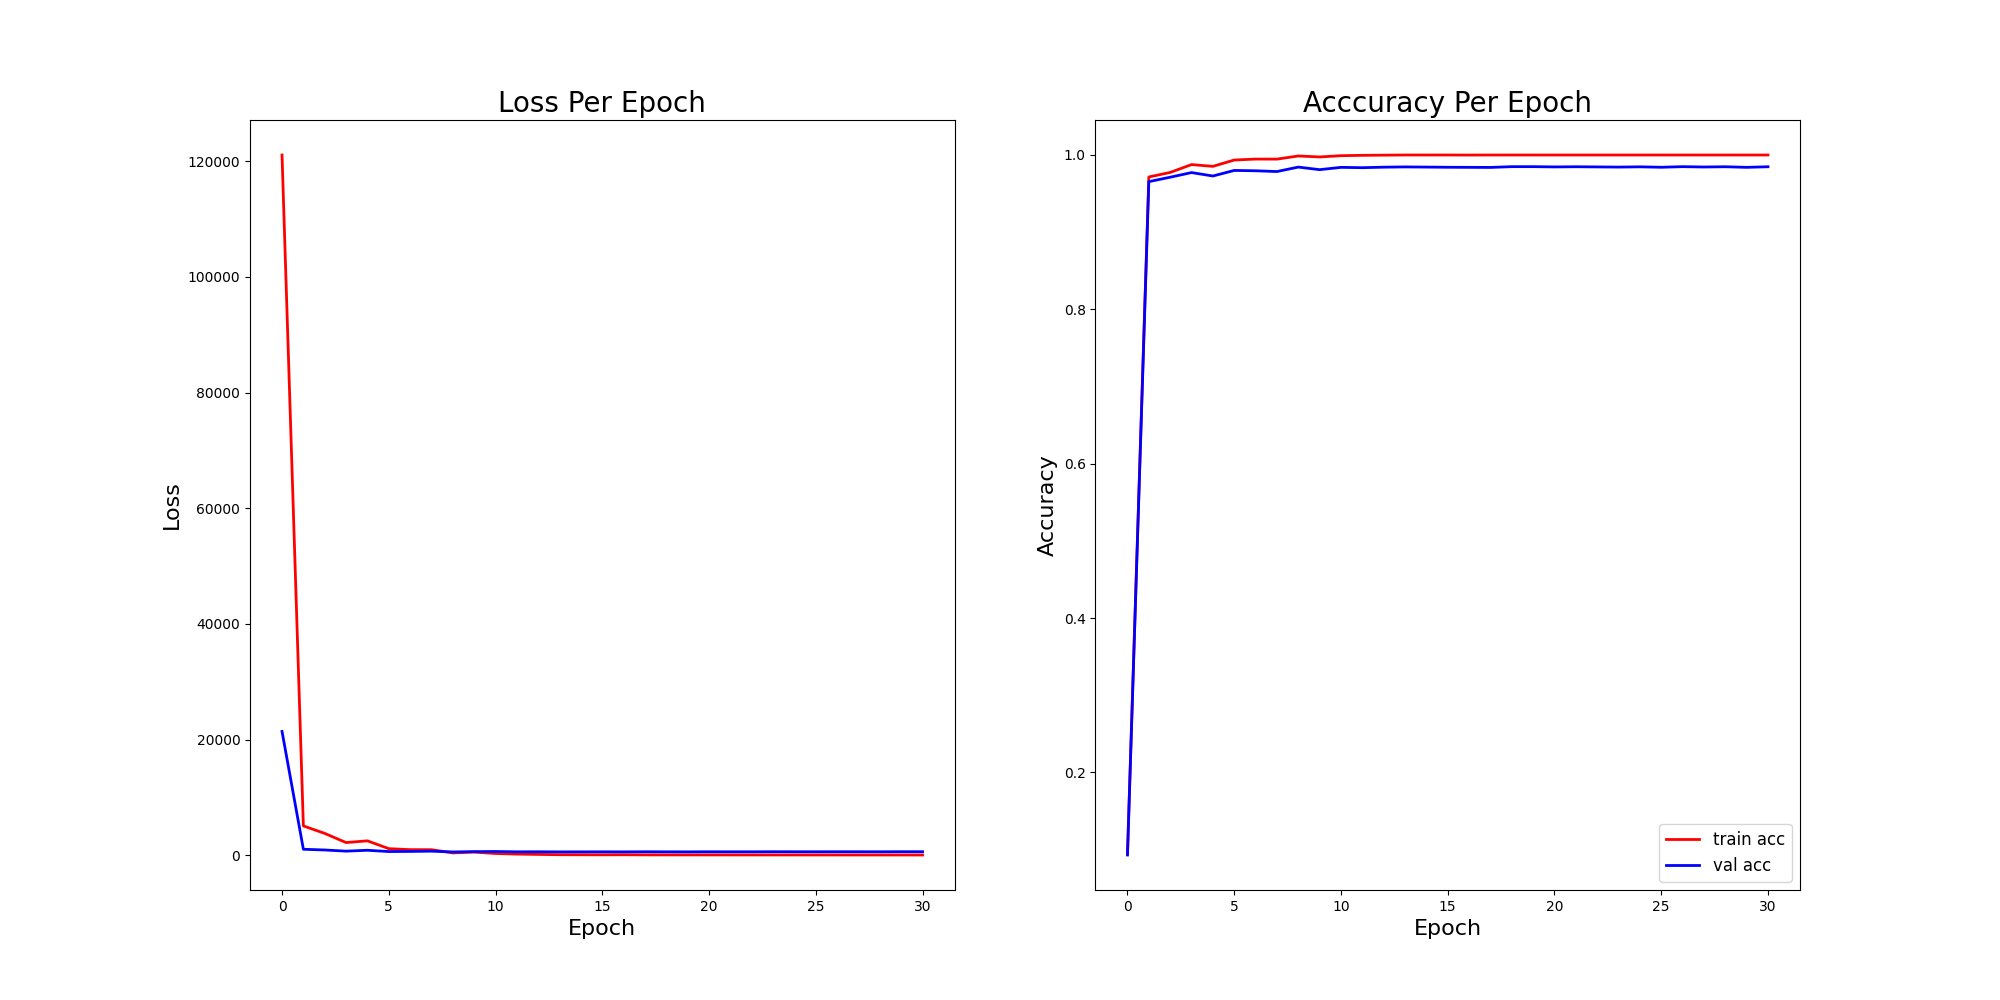
\includegraphics[width=0.8\textwidth]{results/epoch_plots.png}
	\caption{
		Left: Insample (red) and validation (blue) error as a function of epochs. 
		Right: Insample (red) and validation (blue) accuracy as a function of epochs.
		The neural network achieves very low loss after a few epochs.
	}
	\label{fig:error}
\end{figure}
\end{document}